\documentclass[11pt]{article}
\usepackage{pgfplots}
\usepackage[T1]{fontenc}
\usepackage[utf8]{inputenc}
\usepackage{xcolor}
\usepackage{tikz}
\usepackage{pgfplots}
\usepackage{xcolor}
\usepackage{pgfplots}
\usepackage[T1]{fontenc}
\usepackage[utf8]{inputenc}
\usepackage{xcolor}
\usepackage{pgfplots}
\usepackage{colortbl}
\usepackage{amsmath}

\begin{document}

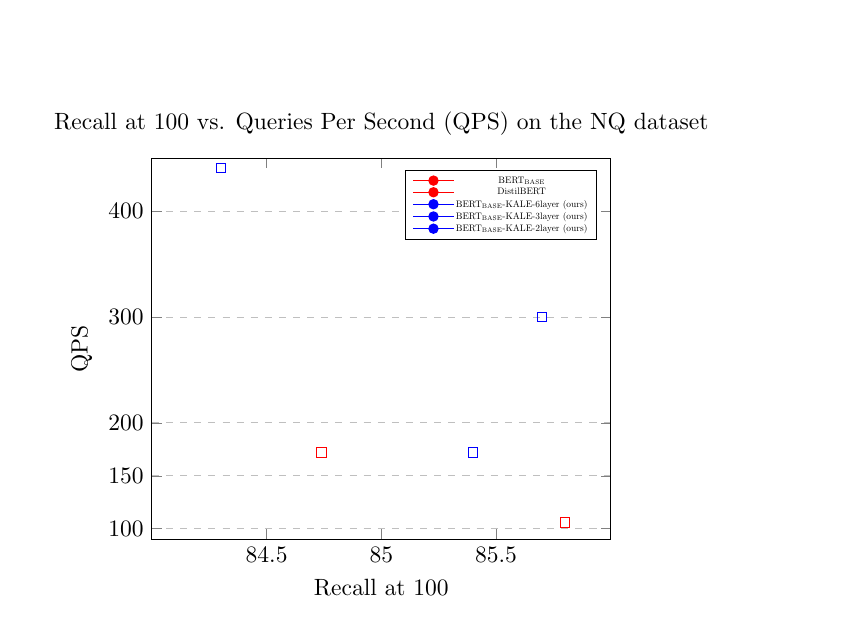
\begin{tikzpicture}
\scalebox{0.85}{
\begin{axis}[
    title={Recall at 100 vs. Queries Per Second (QPS) on the NQ dataset},
    xlabel={Recall at 100},
    ylabel={QPS},
    xmin=84, xmax=86,
    ymin=90 , ymax=450,
    xtick={84.5, 85, 85.5},
    ytick={100, 150, 200, 300,400},
    legend pos=north east,
    ymajorgrids=true,
    grid style=dashed,
    legend style={nodes={scale=0.4, transform shape}}, 
    legend image post style={mark=*}
]
\addplot[
    color=red,
    mark=square,
    ]
    coordinates {
    (85.8,106)
    };

\addplot[
    color=red,
    mark=square,
    ]
    coordinates {
    (84.74,172)
    };
\addplot[
    color=blue,
    mark=square,
    ]
    coordinates {
    (85.4,172)
    };
\addplot[
    color=blue,
    mark=square,
    ]
    coordinates {
    (85.7,300)
    };
\addplot[
    color=blue,
    mark=square,
    ]
    coordinates {
    (84.3,441)
    };

\legend{BERT\textsubscript{BASE}, DistilBERT, BERT\textsubscript{BASE}-KALE-6layer (ours),BERT\textsubscript{BASE}-KALE-3layer (ours), BERT\textsubscript{BASE}-KALE-2layer (ours) }
 \end{axis}}
\end{tikzpicture}

\end{document}